\chapter{Cosmic Microwave Background} \label{ch:cmb}

\section{Introduction} \label{sec:cmb_intro}

\subsubsection{Historical Overview} \label{subsec:cmb_history}

\begin{minipage}{0.46\textwidth}
    The \textbf{cosmic microwave background} (CMB) was theoretically predicted in 1948 by Gamow, Alpher, and Herman, who argued that a Universe originating from a hot, dense state should retain relic thermal radiation, now cooled and stretched by cosmic expansion to populate the microwave portion of the spectrum. This prediction was spectacularly confirmed in 1964, when Penzias and Wilson (working at Bell Labs with an antenna originally designed for satellite research) observed an omnipresent, isotropic excess signal that could not be explained by any known source or interference.
\end{minipage}%
\hfill
\begin{minipage}{0.52\textwidth}
    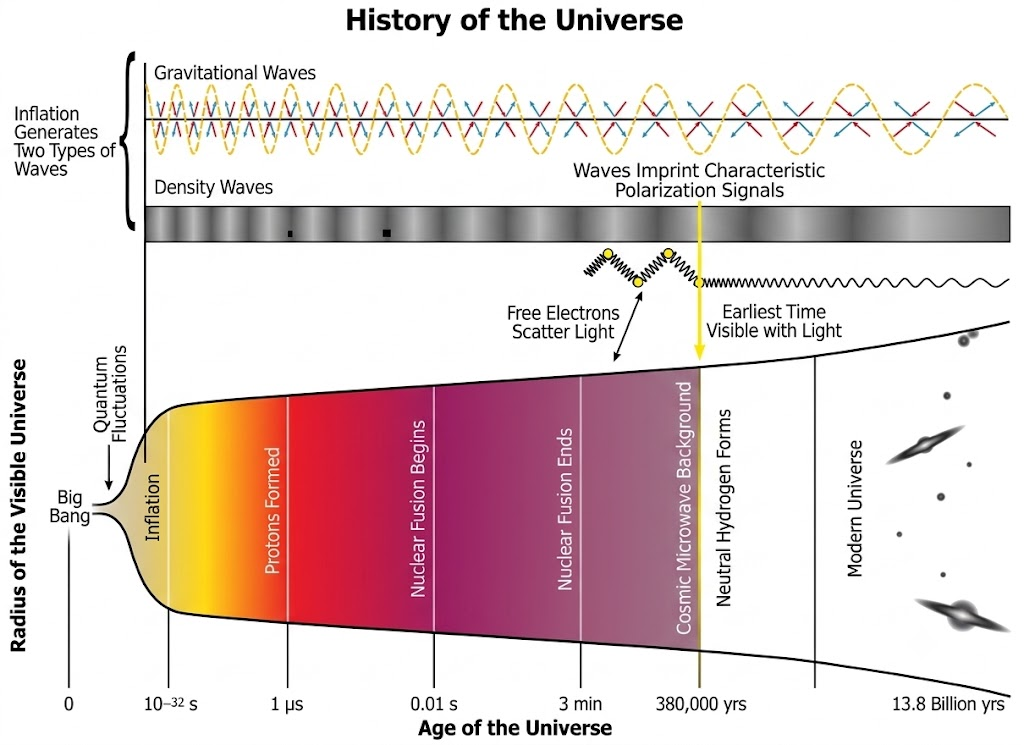
\includegraphics[width=\textwidth]{assets/univ-hist.png}

    \vspace{-0.5em}

    \captionof{figure}{Timeline of the universe \cite{bicep2}.}
    \label{fig:cmb_blackbody}
\end{minipage}

\medskip

\subsubsection{Discovery and detection}

The accidental discovery of the CMB, honoured by the 1978 Nobel Prize, provided decisive evidence for the Big Bang theory and ended serious consideration of the Steady State hypothesis. Over the years, a series of landmark experiments have progressively sharpened our view of the CMB, improving our understanding of the universe's earliest moments.

\medskip

\begin{minipage}{0.54\textwidth}
\begin{itemize}
    \item \textbf{COBE satellite} (1989): Carried out the first full-sky CMB survey, establishing that the CMB is not perfectly smooth but exhibits tiny fluctuations. 
    \item \textbf{BOOMERanG} (1998): A high-altitude balloon launched from Antarctica. With improved angular resolution, it was the first to clearly detect the “first acoustic peak” in the CMB power spectrum.
    \item \textbf{WMAP satellite} (2001): Greatly improved both sensitivity and angular resolution, mapping the full sky and delivering the first full-sky measurements of CMB $E$-mode polarisation.
    \item \textbf{Planck satellite} (2009): Delivered the most detailed image of the CMB to date, measuring the sky's temperature and polarisation (both $E$- and $B$-modes) at multiple frequencies, with an angular resolution 15~times finer than COBE.
\end{itemize}
\end{minipage}%
\hfill
\begin{minipage}{0.43\textwidth}
    \centering
    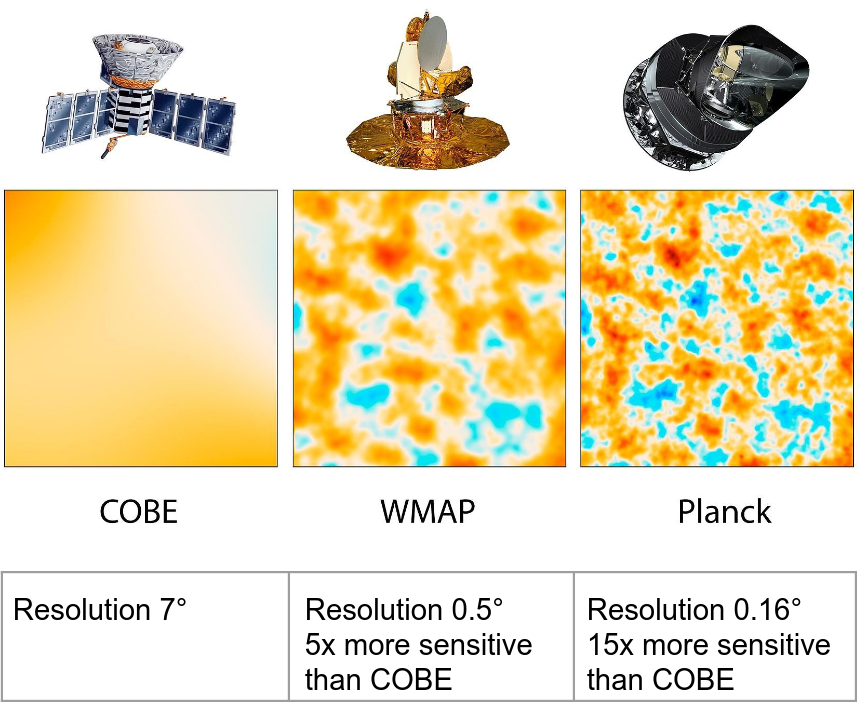
\includegraphics[width=\textwidth]{assets/cmb-obs.png}
    \captionof{figure}{Key CMB observation missions and an example all-sky CMB map.}
    \label{fig:cmb_obs}
\end{minipage}

\section{Properties of the Cosmic Microwave Background} \label{sec:cmb-char}

\subsection{The CMB Monopole and Dipole} \label{subsec:cmb_monopole}

\subsubsection{CMB Monopole}

The CMB spectrum is measured to be an \textbf{almost perfect blackbody} at $T = 2.725\,\text{K}$, as established most precisely by COBE/FIRAS. This exceptional uniformity is a cornerstone of evidence for a hot, thermalised early Universe: any significant late-time energy injection would have left visible distortions from a pure Planck spectrum, yet none have been detected.

\medskip

\begin{center}
    \centering
    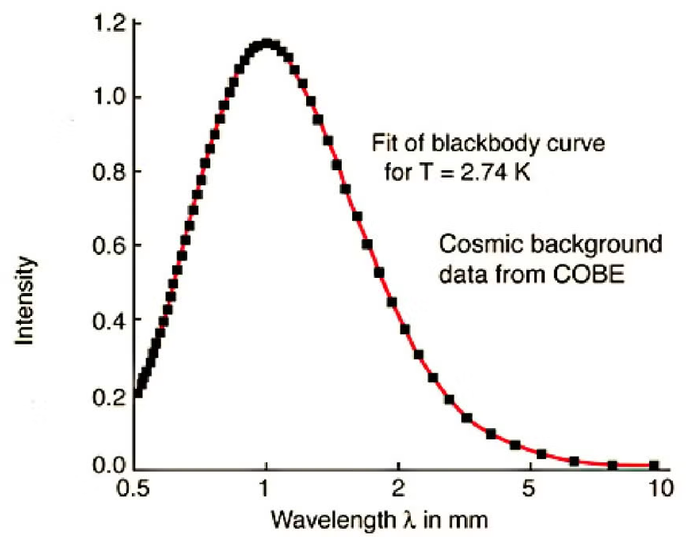
\includegraphics[height=0.2\textheight]{assets/blackbody.png}
    \hspace{4em}
    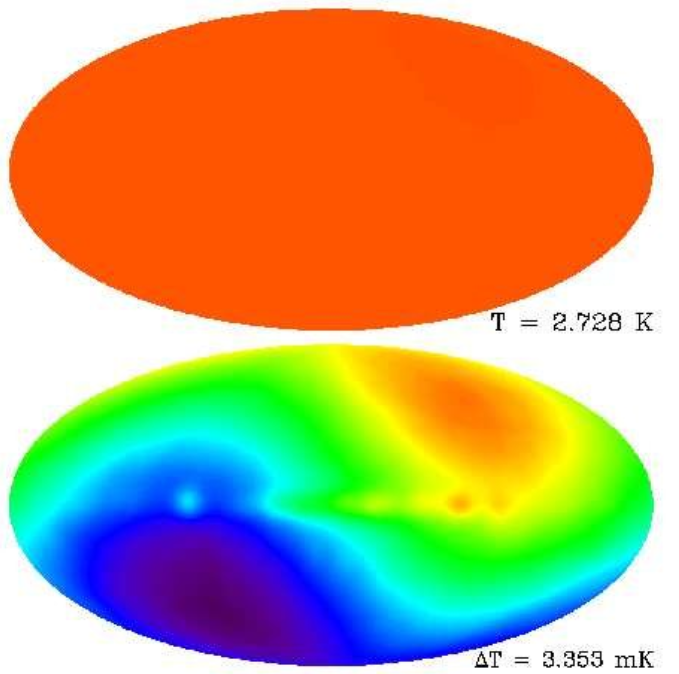
\includegraphics[height=0.22\textheight]{assets/cmb-dipole.png}
    \captionof{figure}{\textbf{Left:} COBE/FIRAS measurement of the CMB spectrum, showing an extremely precise blackbody at $T=2.725$\,K \cite{bb}. \textbf{Right:} The CMB dipole, arising from the Doppler effect due to our motion with respect to the CMB rest frame \cite{garcia}.}
    \label{fig:cmb_blackbody}
\end{center}

% \medskip

\subsubsection{CMB Dipole}

Superposed on the monopole, at the much smaller level of $\Delta T/T \sim 10^{-3}$ (an amplitude of order $3.35\,\text{mK}$), is a dipole pattern: one hemisphere of the sky appears systematically hotter, the opposite one systematically colder. This is a Doppler effect arising from our own peculiar motion through space, which sums the orbital motion of the Earth around the Sun ($\sim 30\,\text{km/s}$), the rotation of the Sun about the Galactic centre ($\sim 220\,\text{km/s}$), and the net motion of the Milky Way toward the Virgo cluster ($\sim 300\,\text{km/s}$); the vector sum of these contributions yields a net peculiar velocity of ${\sim}\,369\,\text{km/s}$. Because the dipole is purely kinematic in origin, it is conventionally subtracted before the intrinsic CMB anisotropies are analysed.

\subsection{CMB Anisotropies} \label{sec:cmb_anisotropies}

\begin{minipage}{0.56\textwidth}
Once the monopole and dipole are removed, the CMB reveals a further layer of structure: tiny temperature fluctuations of order $\Delta T/T \sim 10^{-5}$, remarkably uniform across the sky. These fluctuations originate from quantum effects during inflation, stretched to cosmological scales and imprinted as the seeds of all large-scale structure. Prior to \bfit{recombination}, the tightly coupled baryon-photon fluid resists gravitational collapse through radiation pressure, and the two effects together drive \bfit{acoustic oscillations}: overdense regions collapse under gravity, are halted and rebound under radiation pressure, and the fluid rings much like a sound wave. 
\end{minipage}%
\hfill
\begin{minipage}{0.4\textwidth}
    \centering
    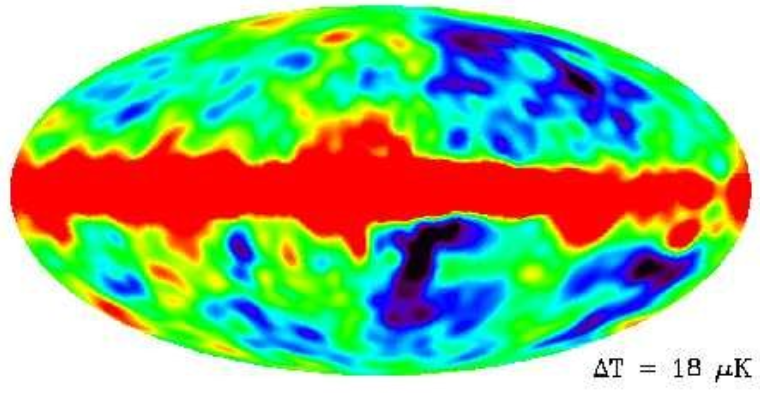
\includegraphics[width=\textwidth]{assets/cmb-anisotropies.png}
    \captionof{figure}{CMB anisotropy map ($\sim$18 $\mu$K) after dipole subtraction.}
    \label{fig:cmb_powerspectrum}
\end{minipage}

\medskip

\begin{minipage}{0.45\textwidth}
    Tiny quantum fluctuations, stretched to cosmic scales by inflation, set the initial density perturbations of the Universe. Prior to recombination, that is, before neutral hydrogen forms, the tightly coupled baryon-photon fluid undergoes acoustic oscillations driven by the interplay of gravity and radiation pressure. As the Universe cools and neutral hydrogen forms at $z \simeq 1100$, photons decouple from baryons and begin to \textbf{free-stream} across the cosmos, largely unimpeded. 

    \medskip

    The temperature pattern we observe in the CMB today is thus a snapshot of these primordial density fluctuations, frozen in at the surface of last scattering.
\end{minipage}%
\hfill
\begin{minipage}{0.53\textwidth}
    \centering
    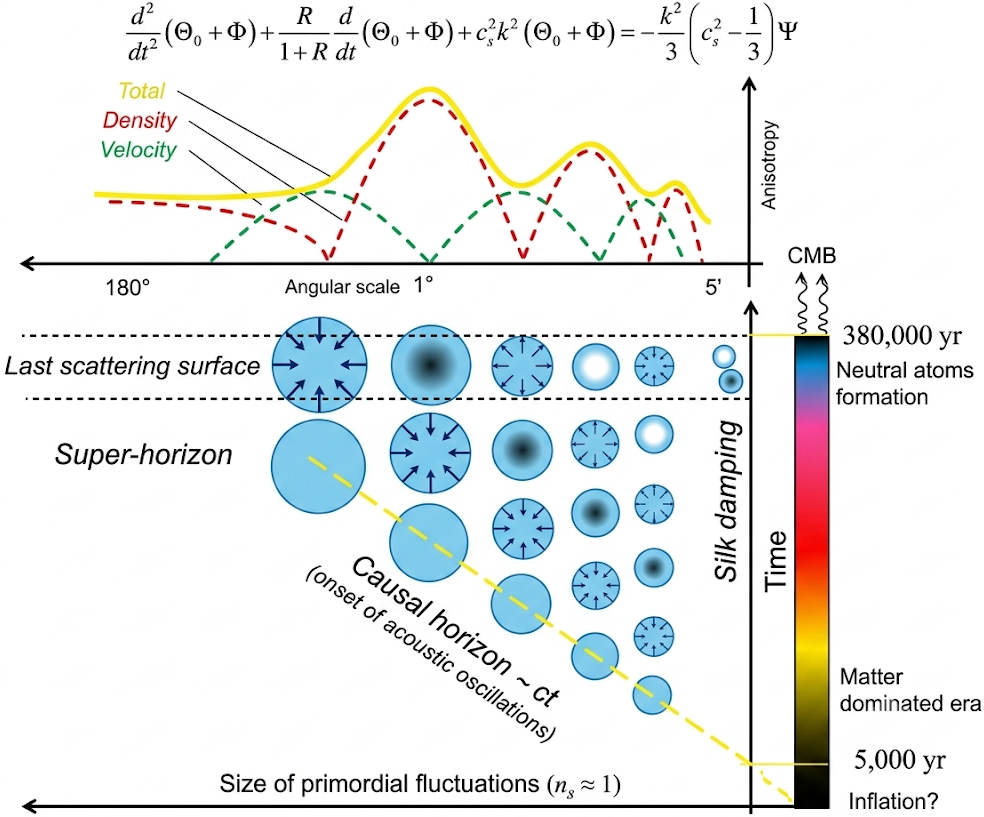
\includegraphics[width=\textwidth]{assets/cmb-acoustic.png}
    \captionof{figure}{Origin of CMB acoustic peaks.}
    \label{fig:cmb_acoustic_origin}
\end{minipage}


\subsubsection{The Angular Power Spectrum} \label{subsubsec:cmb_powerspectrum}

The \textbf{angular power spectrum} encodes both acoustic oscillations on sub-horizon scales and larger super-horizon fluctuations, providing a direct observational imprint of the Universe at the moment of recombination. To analyse the anisotropies statistically, the fractional temperature fluctuation:
$$
\frac{\Delta T}{T}(\theta,\phi) = \frac{T(\theta,\phi) - \bar{T}}{\bar{T}}
$$
is expanded in spherical harmonics,
$$
\frac{\Delta T}{T}(\theta,\phi) = \sum_{\ell=0}^{\infty}\sum_{m=-\ell}^{\ell} a_{\ell m}\, Y_{\ell m}(\theta,\phi) ,
$$
where larger coefficients $a_{\ell m}$ correspond to a stronger contribution from the corresponding mode $Y_{\ell m}$. Because the individual phases carry no physical information for a statistically isotropic random field, the relevant observable is the \bfit{angular power spectrum},
$$
C_\ell = \frac{1}{2\ell+1}\sum_{m=-\ell}^{\ell} \langle |a_{\ell m}|^2 \rangle .
$$
Low multipoles $\ell$ correspond to large angular scales, and increasingly high $\ell$ probes progressively finer angular detail; the sequence of acoustic peaks visible in $C_\ell$ (\cref{fig:cmb_powerspectrum}) directly encodes the oscillation history of the photon-baryon fluid at recombination, and their positions and relative heights constrain essentially all of the fundamental cosmological parameters.

\medskip

\begin{center}
    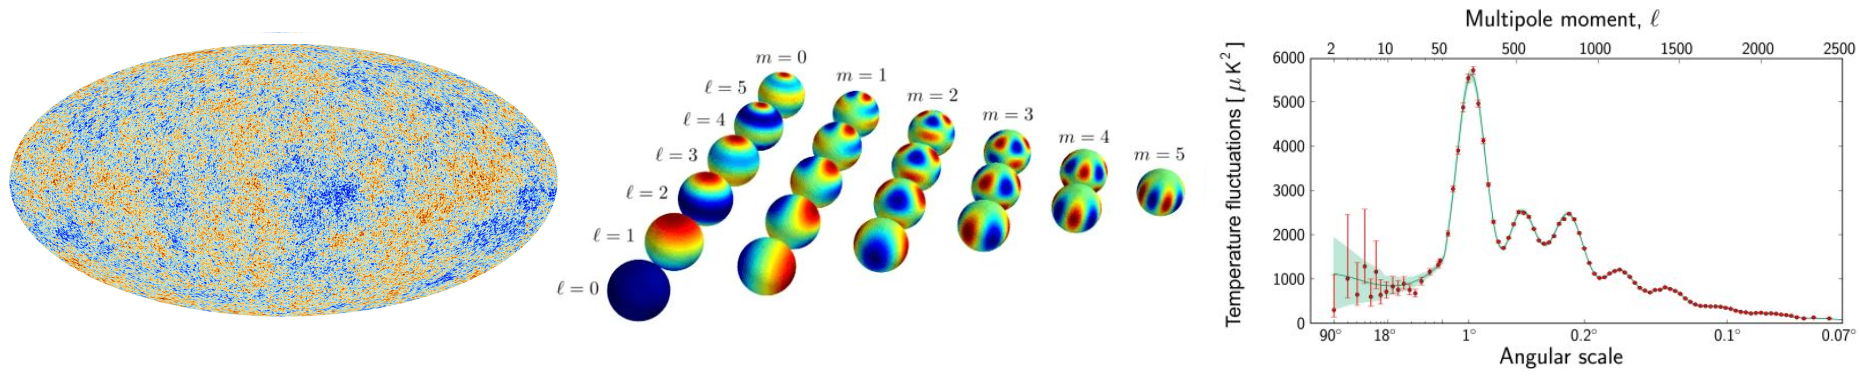
\includegraphics[width=\textwidth]{assets/cmb-anis.png}
    \captionof{figure}{CMB statistical analysis. \textbf{Left:} Full-sky map of temperature anisotropies. \textbf{Middle:} Spherical harmonic modes ($Y_{\ell m}$) showing increasing complexity with higher $\ell$. \textbf{Right:} Measured power spectrum $C_\ell$, with acoustic peaks providing precise cosmological constraints.}
    \label{fig:cmb_powerspectrum}
\end{center}

\begin{observationblock}[Cosmic variance and the limits of temperature measurements]
Because we observe only one Universe, the temperature power spectrum is fundamentally \bfit{sample-variance limited}: with just $(2\ell+1)$ independent modes at each $\ell$, there is an irreducible statistical uncertainty:
$$
\frac{\Delta C_\ell}{C_\ell} = \sqrt{\frac{2}{2\ell+1}} .
$$
This effect is largest at low $\ell$ (large scales), where few modes exist, and decreases as $\ell$ increases. For essentially all scales of cosmological interest ($\ell \lesssim 1500$), Planck was already sensitive enough that cosmic variance (not instrumental noise) sets the dominant uncertainty. Improving temperature measurements further yields little gain; real progress requires probing CMB polarisation, where sample variance does not yet dominate.
\end{observationblock}

\subsection{CMB Polarisation} \label{subsec:cmb_polarization}

\begin{minipage}{0.6\textwidth}

Polarisation in the CMB originates from \textbf{Thomson scattering}. When a free electron is illuminated by incoming radiation, it oscillates along the incident electric field and re-emits linearly polarised light. If this surrounding radiation field is perfectly isotropic, the perpendicular polarisation vectors perfectly cancel out, yielding zero net polarisation. 

\smallskip

A net linear polarisation (at the level of ${\sim}\,10\%$) emerges only if the incident radiation field exhibits a \textbf{quadrupole anisotropy}, meaning its intensity alternates systematically between "hot" and "cold" directions separated by $90^\circ$. Because the electron is driven more strongly by the more intense (hot) radiation, the resulting net polarisation aligns precisely with the orthogonal (cold) axis.
\end{minipage}%
\hfill
\begin{minipage}{0.38\textwidth}
    \vspace{-1em}
    \centering
    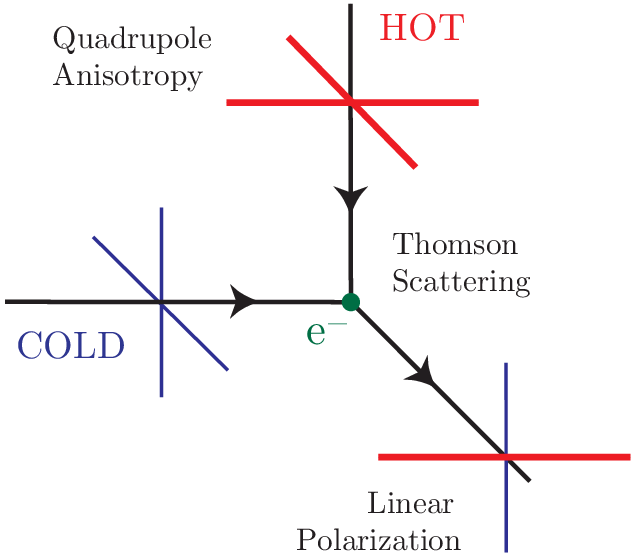
\includegraphics[width=0.9\textwidth]{assets/thomson.png}
    \captionof{figure}{Origin of CMB polarisation through Thomson scattering off a quadrupole radiation field \cite{Baumann}.}
    \label{fig:thomson_polarization}
\end{minipage}

\smallskip

The epoch at which this quadrupole can actually develop is narrowly constrained: before recombination, scattering is far too frequent to allow any significant quadrupole to build up, while after recombination scatterings become extremely rare (until the Universe reionises, \cref{sec:reionization}). Recombination is therefore essentially the only epoch at which CMB polarisation is efficiently generated. Two distinct physical mechanisms can source the required quadrupole: scalar \textbf{density fluctuations} and tensor perturbations due to a stochastic \textbf{gravitational waves} background.

\smallskip

\begin{minipage}{0.62\textwidth}
The linear polarisation pattern we observe across the sky is the imprint of quadrupole anisotropies present at recombination. Because CMB polarisation is a \textbf{spin-2 field}, it can be naturally decomposed into two orthogonal modes:

\smallskip

\begin{itemize}
    \item \textbf{E-mode}: curl-free (gradient-like), polarisation aligned parallel or perpendicular to the wavevector (even parity).
    \item \textbf{B-mode}: divergence-free (curl-like), polarisation tilted at $45^\circ$ to the wavevector (odd parity).
\end{itemize}

\medskip

Importantly, scalar density fluctuations generate only $E$-modes, while tensor perturbations (gravitational waves) can generate both $E$- and $B$-modes. The detection of $B$-modes thus provides a direct signature of a primordial gravitational-wave background and of inflation.
\end{minipage}%
\hfill
\begin{minipage}{0.35\textwidth}
    \centering
    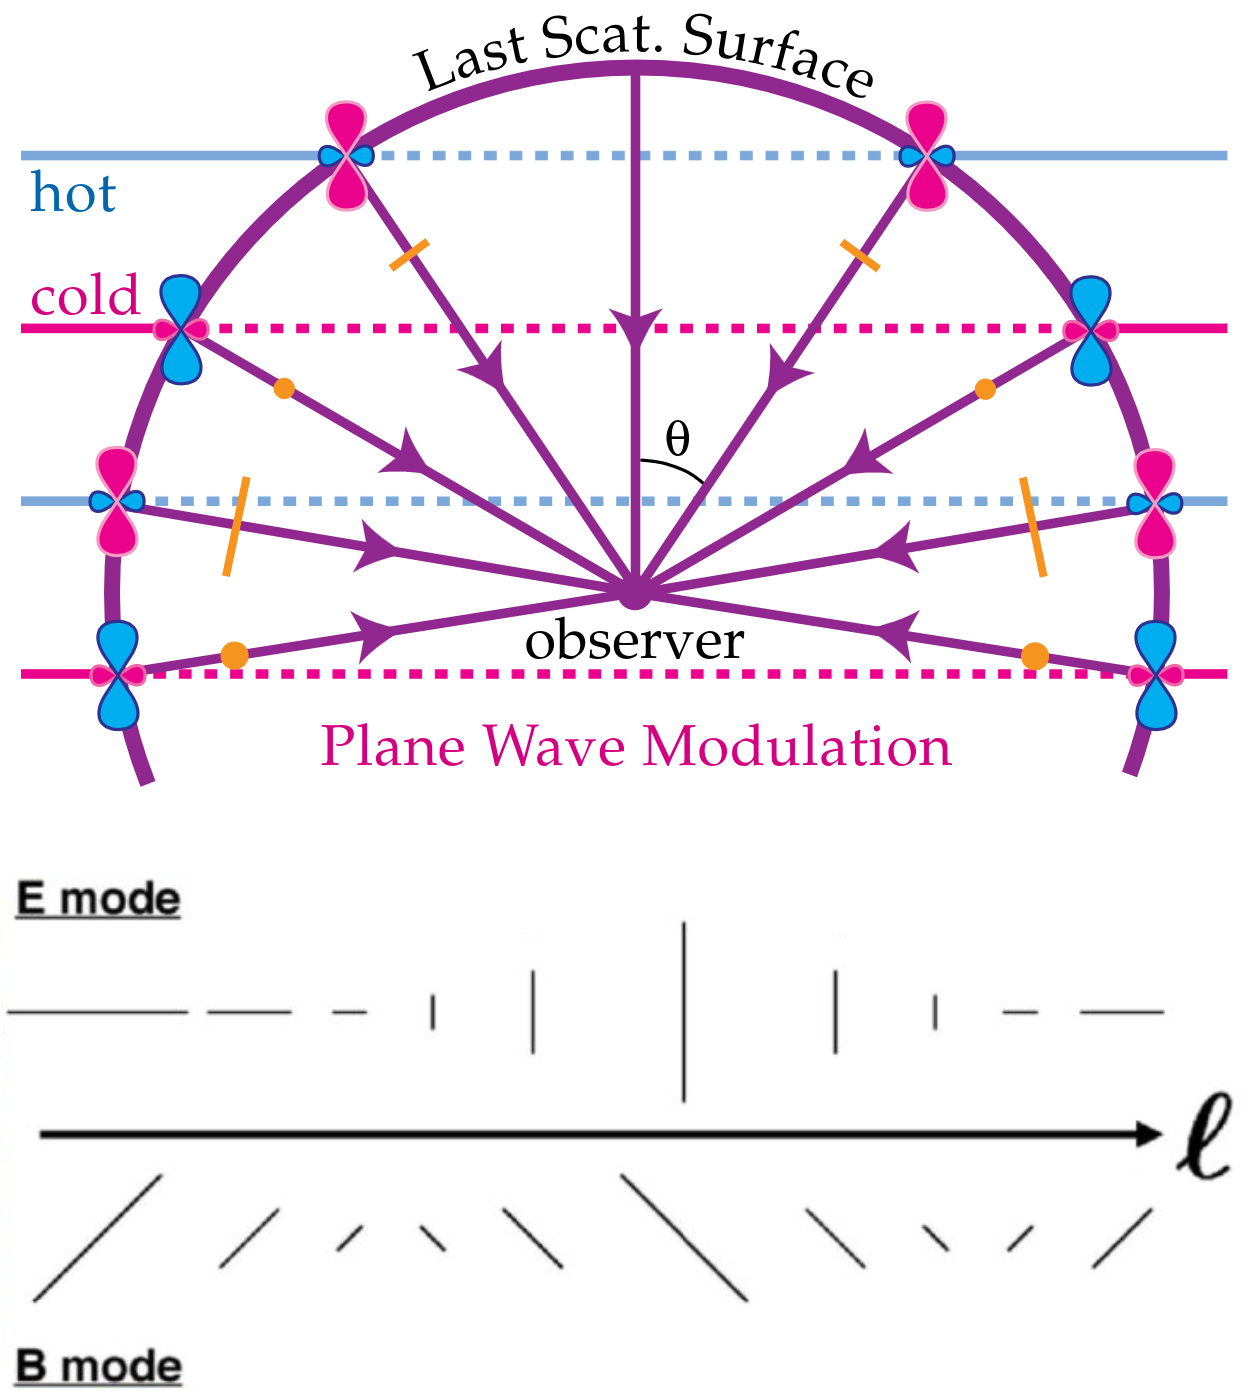
\includegraphics[width=0.9\textwidth]{assets/polarization.png}
    \captionof{figure}{CMB E- and B-mode polarisation patterns \cite{hu}.}
    \label{fig:polebmodes}
\end{minipage}

Standard scalar density perturbations generate both temperature anisotropies and E-mode polarisation, producing three key non-zero power spectra: the auto-correlations $\langle EE \rangle$ and $\langle BB \rangle$, and the cross-correlation $\langle TE \rangle$. In contrast, cross-spectra $\langle EB \rangle$ and $\langle TB \rangle$ must vanish in a parity-conserving Universe, since correlating even-parity (T or E) with odd-parity (B) fields yields a signal that flips sign under mirror reflection, impossible without a preferred handedness.

\medskip

Polarisation signals are much weaker than temperature $\langle TT \rangle$ fluctuations. The $\langle EE \rangle$ spectrum, while small, has been measured down to the sample-variance limit up to $\ell \simeq 3000$. By contrast, the $\langle BB \rangle$ spectrum is extremely faint and noise-limited; its primordial component, a key signature of inflationary gravitational waves, has yet to be detected.

\subsection{Measuring the CMB}

\subsubsection{Foreground Contamination} \label{subsubsec:cmb_foregrounds}

Extracting the CMB signal requires separating it from Galactic foregrounds, principally synchrotron emission (dominant at low frequencies) and thermal dust emission (dominant at high frequencies). In temperature, a narrow "sweet spot" between roughly $70$ and $100\,\text{GHz}$ exists where the CMB dominates over both foregrounds; observations at other frequencies can then be used to characterise and subtract the residual contamination. 

\smallskip

\begin{center}
    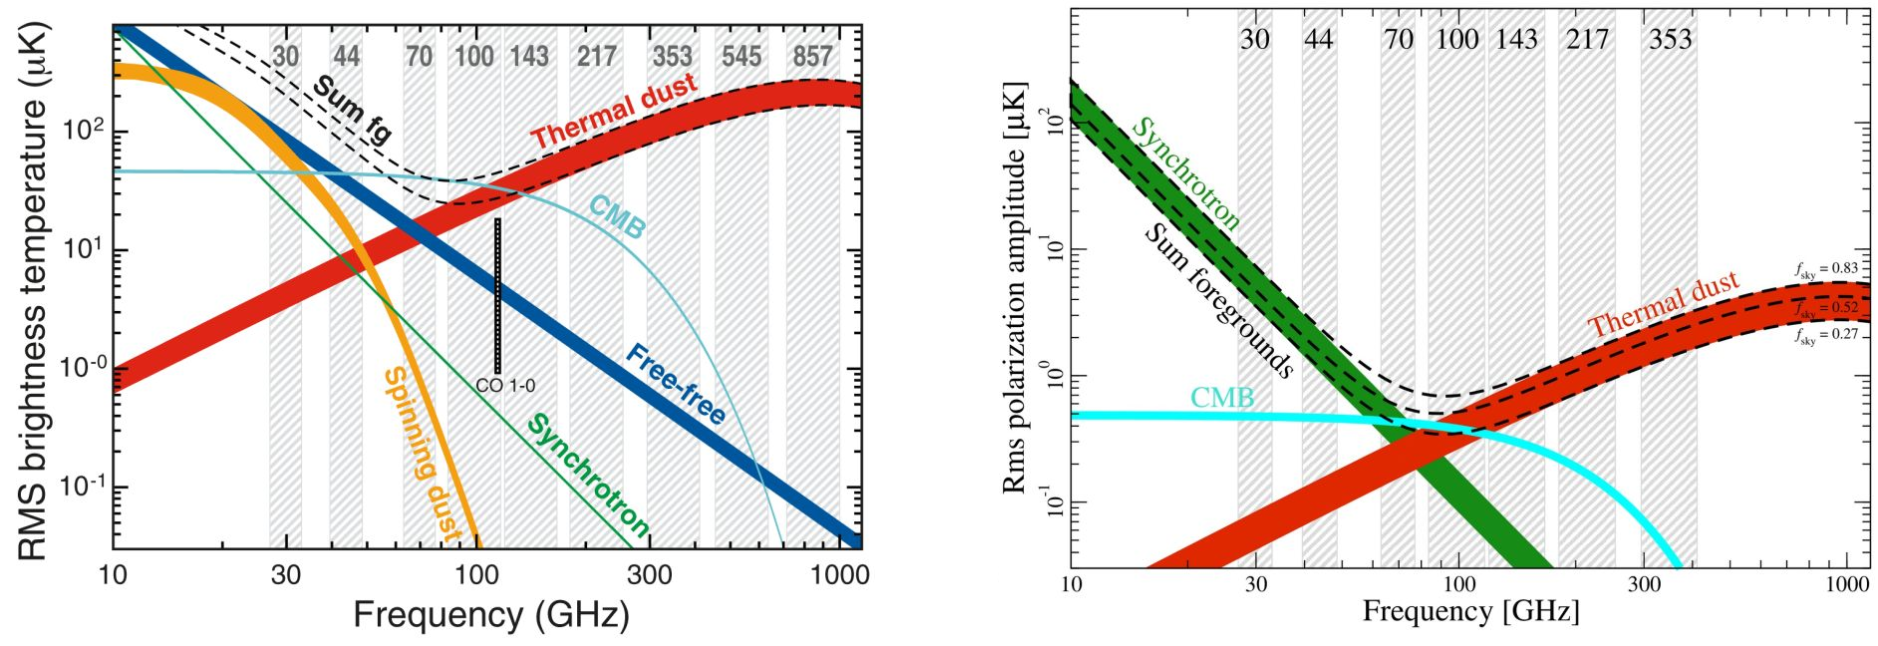
\includegraphics[width=0.8\textwidth]{assets/rms.png}

    \vspace{-0.5em}

    \captionof{figure}{Frequency dependence of CMB and Galactic foregrounds in intensity and polarisation}
    \label{fig:cmb_foregrounds}
\end{center}

\medskip

In polarisation, however, no such clean window exists: synchrotron and dust foregrounds remain comparable to, or brighter than, the CMB polarisation signal across nearly the entire frequency range accessible from the ground or from space, making multi-frequency component separation essential for any polarisation measurement.

\smallskip

\begin{minipage}{0.45\textwidth}
    The \textit{Planck} satellite measured brightness intensity across 9 different frequency bands, and polarisation amplitude in 7 bands (grey vertical bands in \cref{fig:cmb_foregrounds}). Each frequency map reveals distinct types and levels of Galactic foreground emission:

    \smallskip

    \begin{itemize}
        \item \textbf{30-44 GHz}: Emission is dominated by Galactic synchrotron radiation.
        \item \textbf{70-143 GHz}: The CMB signal is strongest relative to foregrounds.
        \item \textbf{217-857 GHz}: Maps are mainly dominated by thermal dust emission, with some contribution from free-free emission.
    \end{itemize}
\end{minipage}%
\hfill
\begin{minipage}{0.52\textwidth}
    \centering
    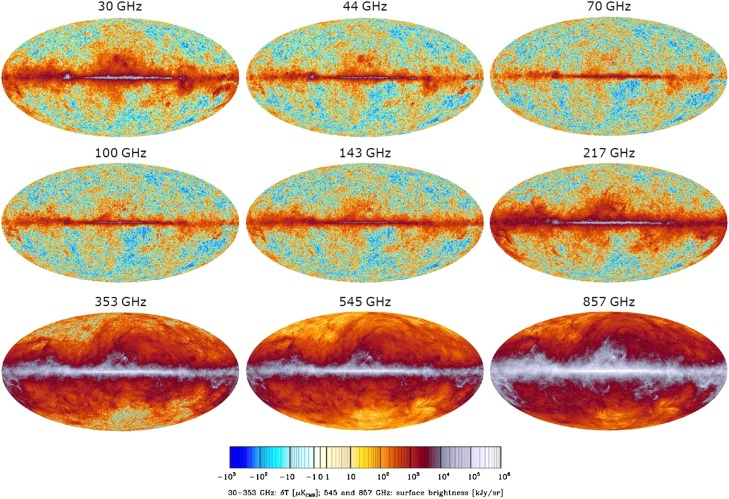
\includegraphics[width=\textwidth]{assets/plank-ons-int.jpg}
    \captionof{figure}{Planck intensity sky maps \cite{plank}.}
    \label{fig:plank-intensity}
\end{minipage}

\medskip

These multi-frequency measurements enable effective separation and characterization of the various foreground components that obscure the CMB signal.

\begin{minipage}{0.55\textwidth}
The polarisation of the CMB is observed through the \textbf{Stokes parameters} $Q$ and $U$, which specify the linear polarisation state of the radiation at every point on the sky. For any direction $\hat{\theta}$:
\begin{itemize}
    \item $Q$ measures the intensity difference between polarisations aligned along the $0^\circ$ and $90^\circ$ axes (i.e., North-South vs.\ East-West).
    \item $U$ quantifies the intensity difference between polarisations at $45^\circ$ and $135^\circ$.
\end{itemize}
Together, $Q$ and $U$ encode the amplitude and direction of the projected electric field vector, and can be transformed into the $E$- and $B$-mode pattern maps for physical interpretation and analysis.
$$
\begin{array}{rl}
\displaystyle Q(\hat\theta) &\displaystyle = \int \frac{d^2\ell}{(2\pi)^2} \left[ E_{\ell}\cos 2\phi_{\ell} - B_{\ell}\sin 2\phi_{\ell} \right] e^{i\ell\cdot\hat\theta} \\
\displaystyle U(\hat\theta) &\displaystyle = \int \frac{d^2\ell}{(2\pi)^2} \left[ E_{\ell}\sin 2\phi_{\ell} + B_{\ell}\cos 2\phi_{\ell} \right] e^{i\ell\cdot\hat\theta}
\end{array}
$$

The total observed polarised intensity is given by:

$$
P = \sqrt{Q^2 + U^2}
$$

\end{minipage}%
\hfill
\begin{minipage}{0.43\textwidth}
    \centering
    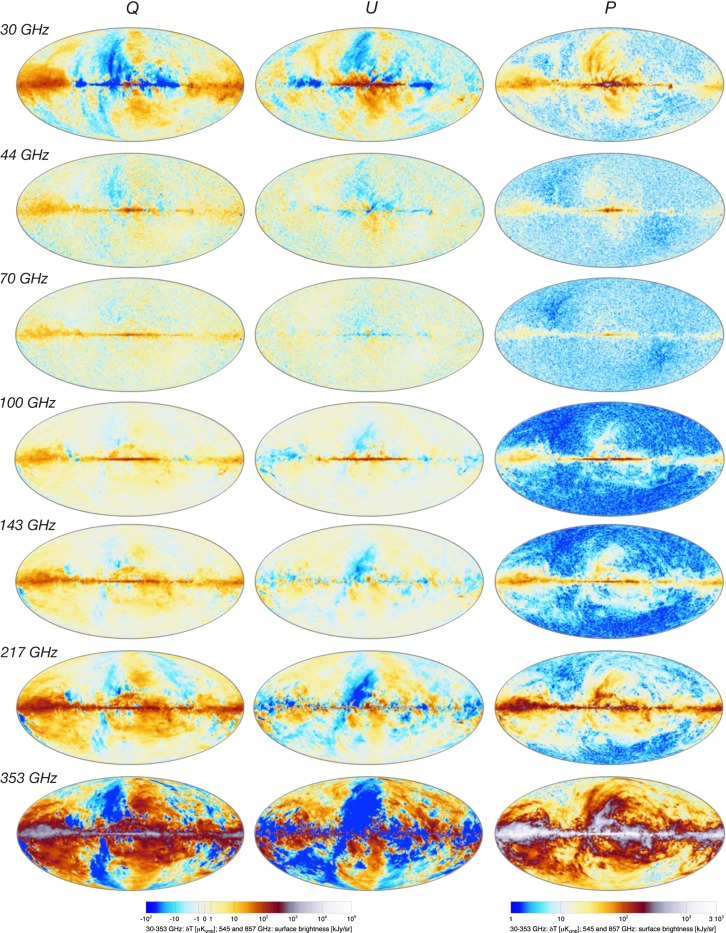
\includegraphics[width=0.97\textwidth]{assets/plank-obs-pol.jpg}
    \captionof{figure}{Planck polarisation sky maps. Each row shows the sky maps of Stokes $Q$ and $U$ at a specific frequency \cite{plank}.}
    \label{fig:plank-polarised}
\end{minipage}

\medskip

This formalism allows us to analyze the detailed structure and frequency dependence of CMB polarisation and foregrounds across the sky, as revealed in the Planck $Q$ and $U$ maps \cref{fig:plank-polarised}.

\subsubsection{The Search for Primordial $B$~modes} \label{subsubsec:cmb_bmodes}

\begin{minipage}{0.42\textwidth}
    
    Studying the CMB allows us to look back to the first epoch in the universe accessible to electromagnetic waves: recombination. At this time, the universe became transparent and photons began to travel freely, giving rise to the oldest light we can observe today. 

    \medskip
    
    The $B$-modes in CMB polarisation carry unique information about gravitational waves produced during inflation. By examining their distribution, we can gain insights into the conditions of the universe even before the era of recombination.
\end{minipage}%
\hfill
\begin{minipage}{0.55\textwidth}
    \vspace{-1em}
    \centering
    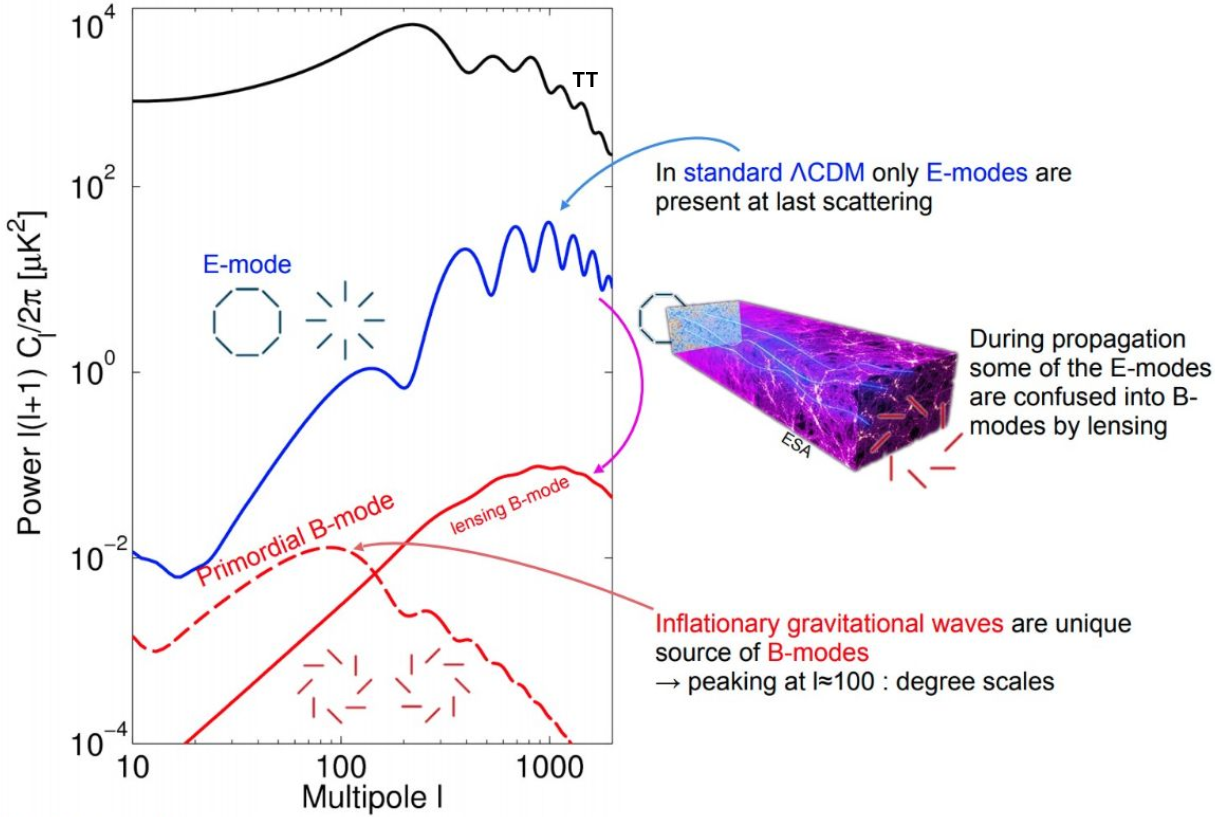
\includegraphics[width=\textwidth]{assets/bicep2.png}

    \vspace{-0.5em}

    \captionof{figure}{Characteristic $E$- and $B$-mode CMB polarisation patterns and their power spectra.}
    \label{fig:cmb_bicep2}
\end{minipage}

\medskip

An important complication is that gravitational lensing by intervening large-scale structure can distort primordial $E$-mode polarisation, partially converting it into $B$-modes. These lensing-induced $B$-modes dominate the $B$-mode signal at smaller angular scales ($\ell \gtrsim 100$), whereas the primordial inflationary $B$-modes are expected to peak at larger angular scales.

\medskip

Within the simplest single-field inflationary models, the amplitude of the primordial $BB$ power spectrum, peaking at degree scales ($\ell \sim 100$), is controlled by a single parameter, the \textbf{tensor-to-scalar ratio} $r$. Because no high angular resolution is required to probe these large scales, dedicated $B$-mode experiments favour large numbers of low-noise detectors over fine angular resolution. Early searches yielded only upper limits: BICEP1 set a $2\sigma$ bound of $r < 0.7$ in 2014.

\begin{observationblock}[The BICEP2 dust controversy]
\textbf{BICEP2} was designed to detect primordial $B$~modes, operating at $150\,\text{GHz}$ near the CMB peak and targeting the "Southern Hole" (then thought to be unusually free of Galactic dust) with an estimated foreground contribution of only $r < 0.01$. In 2014, BICEP2 reported a significant excess in the $BB$ spectrum, inferring $r = 0.20^{+0.07}_{-0.05}$ and ruling out $r=0$ at $7\sigma$.

\smallskip

However, subsequent Planck dust maps at $353\,\text{GHz}$ (unavailable during the initial BICEP2 analysis) revealed that polarised dust emission in the BICEP2 region was far stronger than anticipated, approximately $20\times$ higher at $353\,\text{GHz}$ than at $150\,\text{GHz}$. A combined analysis incorporating both BICEP2/Keck and Planck observations enabled a more accurate subtraction of the dust signal, resulting in an updated upper limit of $r_{0.05} < 0.12$ ($95\%$ confidence), eliminating evidence for a primordial detection. This experience highlighted the risks of claiming a cosmological discovery from a single frequency band, while also underscoring the importance and effectiveness of multi-frequency foreground analysis.
\end{observationblock}

The most recent constraints, combining Planck, BICEP/Keck (through the 2018 season, "BK18"), and baryon acoustic oscillation and lensing data, place the bound at $r < 0.037$ ($2\sigma$), already sufficient to rule out several of the simplest, historically favoured single-field inflationary potentials. $B$-mode detection remains the primary science driver of the next generation of CMB experiments (CMB-S4, the Simons Observatory, LiteBIRD, described in \cref{sec:mm_cmb}), which aim to reach $\mu\text{K}$-arcmin sensitivity in polarisation over nearly the full sky.

\section{The Epoch of Reionization} \label{sec:reionization}

\subsection{Cosmic Timeline} \label{subsec:reionization_timeline}

After the last scattering epoch ($z \simeq 1100$, $t \simeq 380\,000\,\text{yr}$), the Universe enters the \textbf{Dark Ages}: matter is almost entirely neutral, and no astrophysical sources yet exist to emit ionising photons. The Dark Ages end with the formation of the first stars, at redshifts thought to lie around $z \sim 15$-$30$. As increasingly numerous sources of ultraviolet radiation switch on, isolated ionised bubbles form around them, grow, and eventually overlap, marking the \textbf{epoch of reionization} proper ($z \sim 6$-$15$); by $z \sim 6$ the intergalactic medium (IGM) is essentially fully ionised, and the subsequent Post-Reionization era is dominated by the assembly of galaxies observed today. Because the low-redshift Universe is strongly shaped by subsequent astrophysical (baryonic) processes, the reionization epoch offers a comparatively clean window onto the properties of the first luminous sources and the growth of large-scale structure.

\smallskip

\begin{center}
    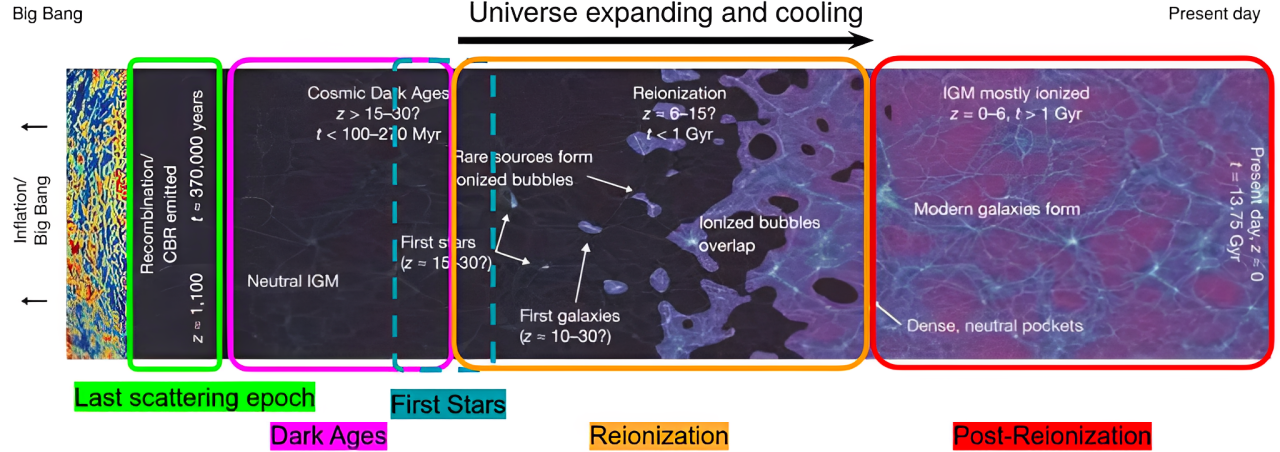
\includegraphics[width=\textwidth]{assets/uni-hist.png}
    \captionof{figure}{Schematic timeline of the universe history.}
    \label{fig:reionization_timeline}
\end{center}

The 21\,cm line from neutral hydrogen during the Dark Ages could, in theory, reveal much about this hidden epoch. Cosmic expansion shifts this line to 10-100\,MHz today, frequencies inaccessible to ground-based telescopes, since Earth's ionosphere blocks them. Even above this range, human-made radio interference is severe, complicating observations for both ground and orbital instruments. A promising solution is to deploy radio telescopes on the far side of the Moon, shielded from both terrestrial interference and the ionosphere, enabling direct study of the redshifted 21\,cm signal.

\begin{tipsblock}[Significance of the Dark Ages]
    At present, the "dark ages" of our universe remain inaccessible to direct astronomical observation. Nevertheless, this epoch is crucial for cosmology: during the dark ages, density perturbations evolved in the linear regime, making this period more tractable for theoretical study. In contrast, the later universe is dominated by complex astrophysical processes that introduce significant non-linearities and modeling challenges.
\end{tipsblock}

\subsection{Evidence from the CMB} \label{subsec:reionization_cmb}

CMB photons that traverse the reionized IGM after last scattering have a non-negligible probability of Thomson-scattering off the newly liberated free electrons. The relevant observable is the \textbf{optical depth to reionization}:
$$
\tau = \int_0^{z_{\text{re}}} n_e(z)\,\sigma_{\mathrm T}\, \frac{c\,dz}{(1+z)H(z)}
$$
where $n_e(z)$ is the free-electron density and $H(z)$ the Hubble parameter; because the IGM is essentially neutral at $z > z_{\text{re}}$, the integral effectively receives contributions only from the epoch of reionization itself, down to the present.

\smallskip

Since this additional scattering is a random process along the line of sight, it does not imprint new structure but rather isotropically damps the primary temperature fluctuations at all angular scales:

\smallskip

\begin{minipage}{0.55\textwidth}
$$
C_\ell^{TT,\text{obs}} = e^{-2\tau}\, C_\ell^{TT,\text{primordial}}
$$

This damping is, however, degenerate with the amplitude of the primordial density fluctuations (parametrised by $A_s$ or $\sigma_8$), since both suppress or enhance the observed spectrum in a very similar way:

$$
C_\ell^{TT,\text{obs}} \propto A_s\, e^{-2\tau}
$$

The degeneracy can be broken using the $TE$ temperature-polarisation cross-spectrum: reionization polarises CMB photons for the first time since recombination, producing a distinctive "bump" at large scales ($\ell \lesssim 10$) that has no counterpart in $A_s$ alone.
\end{minipage}%
\hfill
\begin{minipage}{0.42\textwidth}
    \centering
    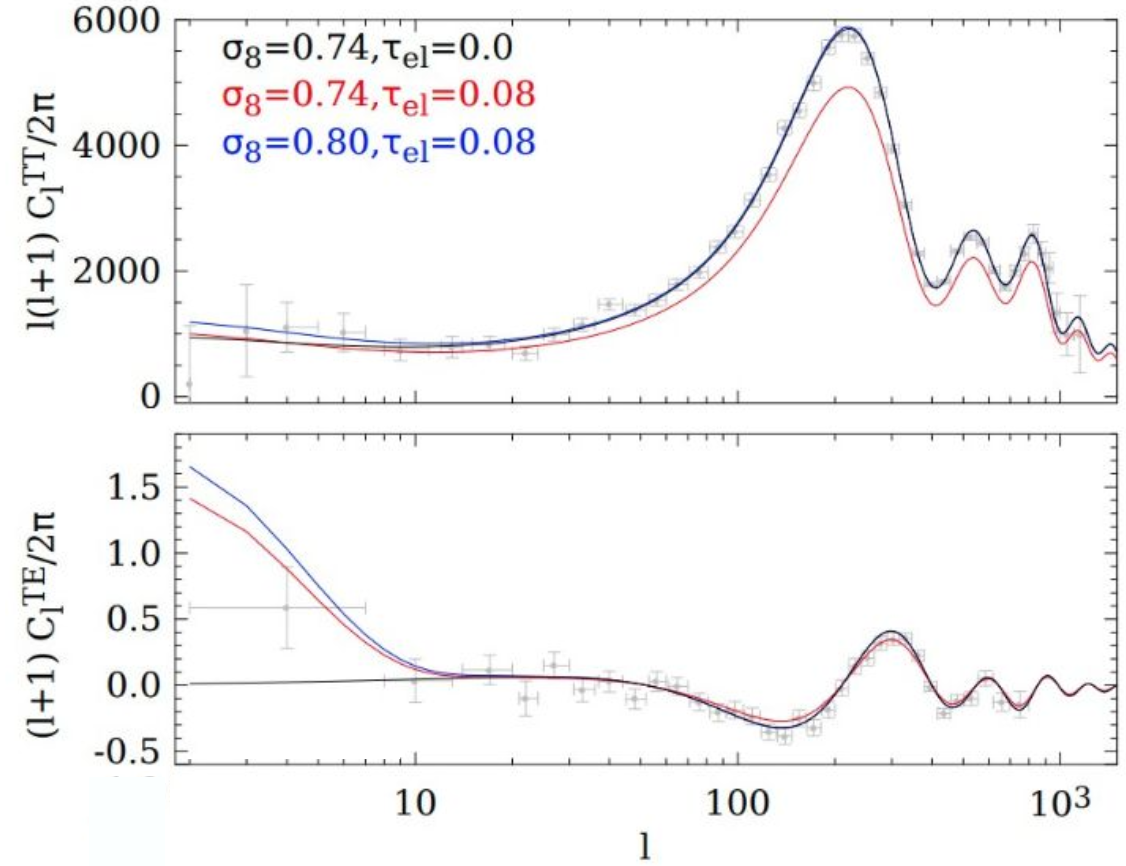
\includegraphics[width=\textwidth]{assets/cmb-scattering.png}

    \vspace{-0.5em}

    \captionof{figure}{Effect of varying the optical depth $\tau$ and amplitude $\sigma_8$ on the CMB angular power spectra (TT and TE).}
    \label{fig:cmb_scattering}
\end{minipage}

\smallskip

Extracting $z_{\text{re}}$ in practice requires assuming a model for the reionization history $n_e(z)$. The simplest and most widely used is the \textbf{instantaneous reionization} model, in which the ionisation fraction transitions from neutral ($n_e = n_H^{\phantom{ }}$) to fully ionised ($n_e = 0$) over a narrow redshift interval ($\Delta z_{\text{re}} \simeq 0.5$) following a symmetric hyperbolic-tangent profile:
$$
x_e(z) = \frac{1+f_{\text{He}}}{2}\left[1 + \tanh\!\left(\frac{(1+z_{\text{re}})^{3/2} - (1+z)^{3/2}}{\Delta w}\right)\right] .
$$

Current Planck constraints, under this simplified model, give $z_{\text{re}} \simeq 7.7$.

\subsection{The Lyman-$\alpha$ Forest} \label{subsec:lyman_alpha}

A particularly direct and independent probe of the ionisation state of the intergalactic medium (IGM) comes from the spectra of distant sources (typically QSOs). 

\begin{minipage}{0.58\textwidth}
As the light travels toward us, any intervening cloud of neutral hydrogen along the line of sight will selectively absorb photons at the rest-frame Lyman-$\alpha$ wavelength, $\lambda_{\text{fi}} = 1216\,\text{\AA}$. However, due to the cosmic expansion, photons emitted with $\lambda_Q < \lambda_{\text{fi}}$ by the source gradually redshift until they match the resonant condition for Lyman-$\alpha$ absorption in a neutral hydrogen cloud at some redshift $z$ ($z < z_Q$), generating an absorption feature in the observed spectrum. The resonance condition at redshift $z$ is:

$$
\frac{\nu_Q}{1+z_Q} = \frac{\nu_{\text{fi}}}{1+z} \quad \Rightarrow \quad \lambda_Q(1+z_Q) = \lambda_{\text{fi}}(1+z)
$$
\end{minipage}%
\hfill
\begin{minipage}{0.4\textwidth}

    \vspace{-0.2em}

    \centering
    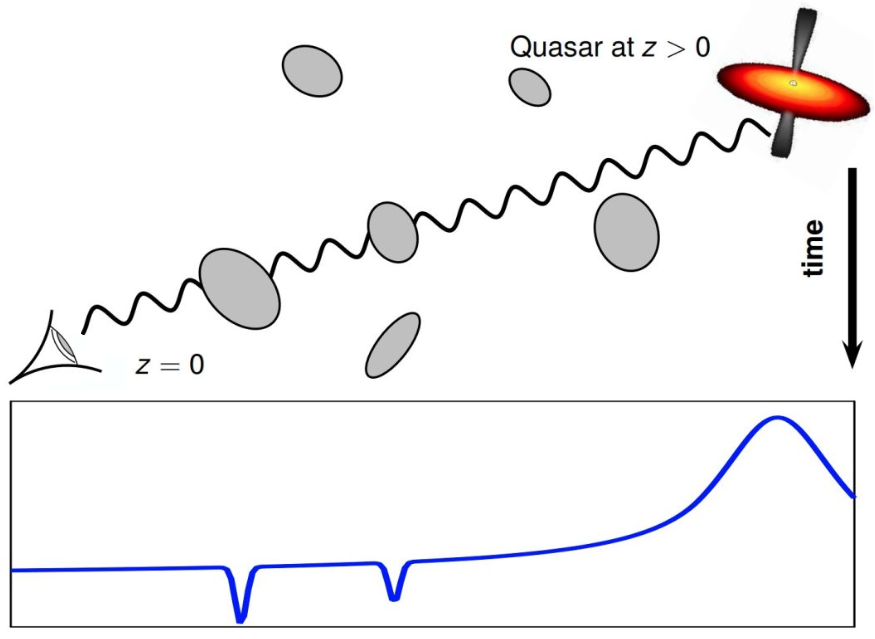
\includegraphics[width=0.95\textwidth]{assets/lyman.png}

    \vspace{-0.5em}

    \captionof{figure}{Origin of the Lyman-$\alpha$ forest: absorption of QSO light by intervening neutral hydrogen.}
    \label{fig:lyman_alpha_forest}
\end{minipage}

\medskip

The dense forest of such absorption features shortward of the QSO's own Lyman-$\alpha$ emission line, produced by the many discrete clouds of neutral hydrogen along the line of sight, gives the phenomenon its name: the \bfit{Lyman-$\alpha$ forest}.

\begin{exampleblock}[Redshift of a Lyman-$\alpha$ absorber]
Consider a QSO at $z_Q = 3$ emitting a photon at rest-frame wavelength $\lambda_Q = 1187\,\text{\AA} < \lambda_{\text{fi}}$. This photon redshifts into resonance with the Lyman-$\alpha$ transition, $\lambda_{\text{fi}} = 1216\,\text{\AA}$, at an intervening redshift
$$
z \simeq 1187 \times \frac{1+z_Q}{1216} - 1 = 1187 \times \frac{4}{1216} - 1 \simeq 2.9 .
$$
If neutral hydrogen is present at that location along the line of sight, it imprints a distinct absorption feature. This feature is observed today, redshifted all the way from the QSO, at:

$$
\lambda_{\text{obs}} = \lambda_Q(1+z_Q) \simeq 1187 \times 4 \simeq 4742\,\text{\AA} .
$$
\end{exampleblock}

More generally, absorption occurring at any intervening redshift $z$ will appear at a corresponding observed wavelength $\lambda_{\text{obs}} = \lambda_{\text{fi}}(1+z)$ in the QSO spectrum. As a result, each quasar spectrum displays a \bfit{forest} of absorption lines blueward of its intrinsic Lyman-$\alpha$ emission peak: these are imprinted by clouds of neutral hydrogen located between the observer and the QSO. 

\smallskip

\begin{minipage}{0.5\textwidth}
The density of absorption features directly traces the distribution and abundance of neutral hydrogen in the intergalactic medium (IGM) along the line of sight: the unabsorbed regions of the spectrum either reflect ionized regions where neutral hydrogen is absent, or simply empty space. This ensemble of closely spaced absorption lines is collectively referred to as the \textit{Lyman-$\alpha$ forest}, as illustrated in \cref{fig:lyman_forest_example}: at low redshift the forest is sparse, while at high redshift the density of absorption lines rises dramatically, reflecting the increasing neutral hydrogen fraction in the early universe.
\end{minipage}%
\hfill
\begin{minipage}{0.47\textwidth}

    \centering
    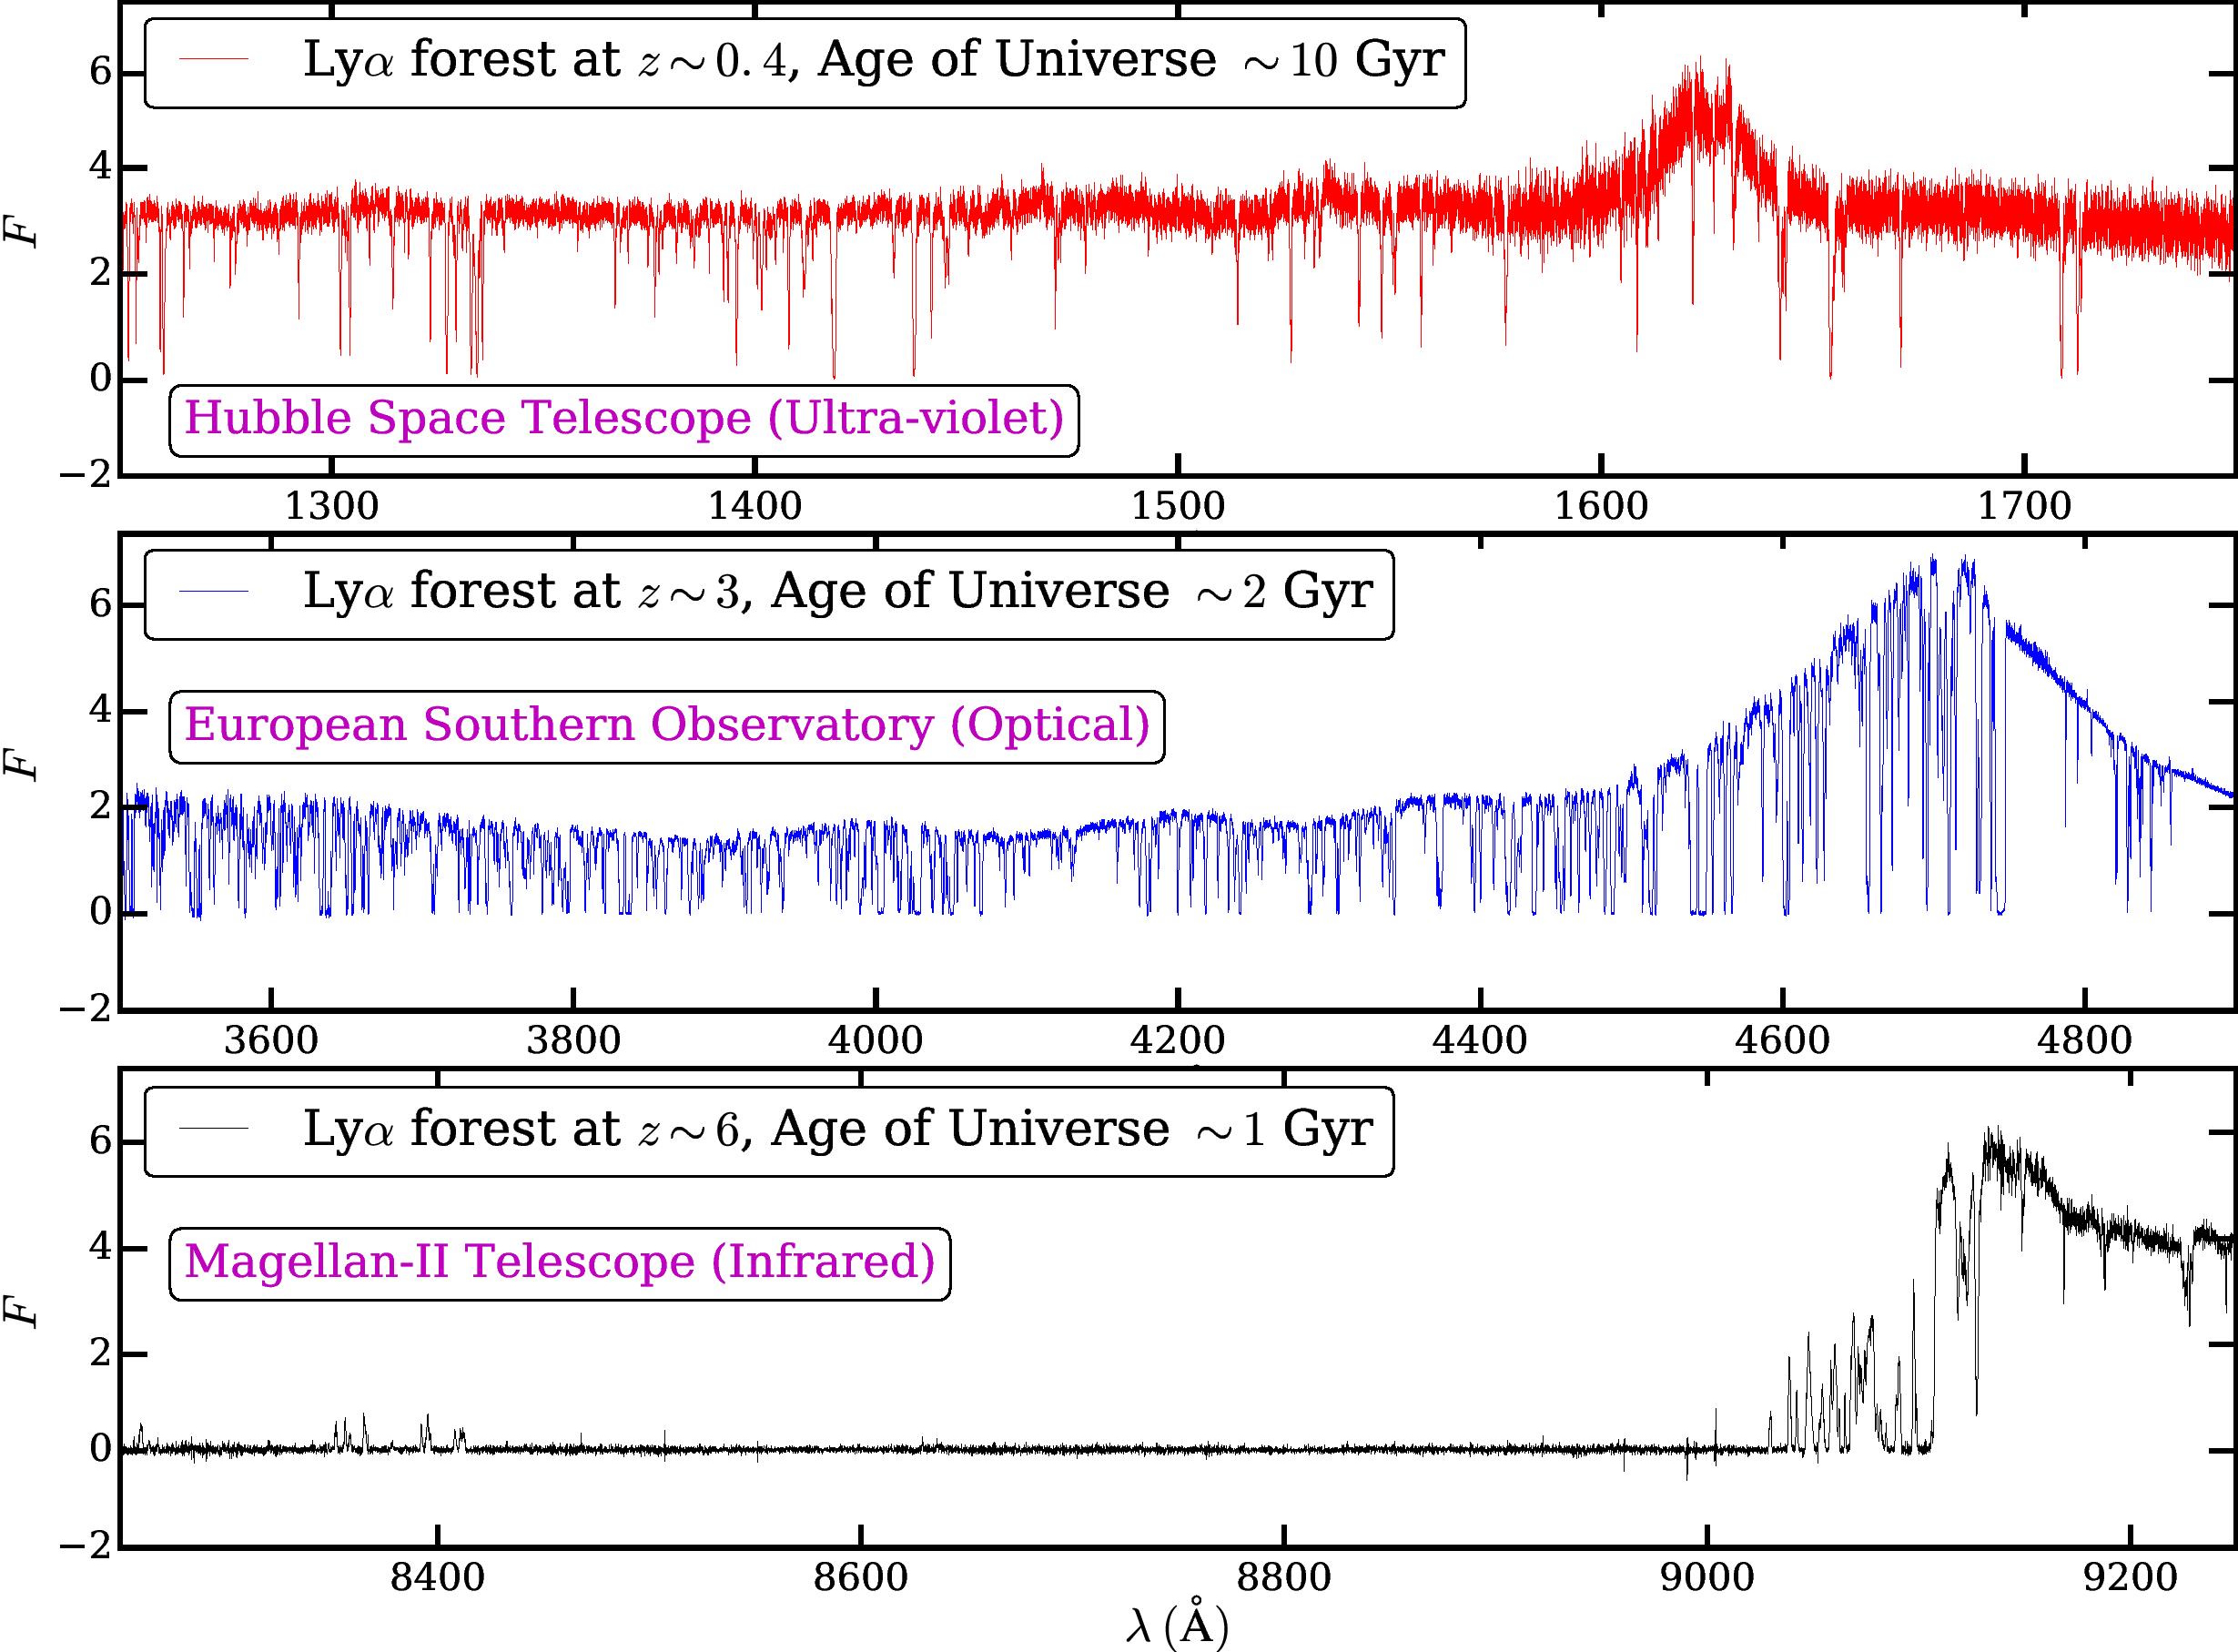
\includegraphics[width=\textwidth]{assets/lyman-ex.jpg}

    \vspace{-0.5em}

    \captionof{figure}{Observed Lyman-$\alpha$ forest at different redshifts \cite{kicc_igm_evolution}.}
    \label{fig:lyman_forest_example}
\end{minipage}

\subsubsection{The Gunn-Peterson Effect} \label{subsec:gunn_peterson}

If before reionization the IGM was filled with neutral hydrogen, essentially every wavelength blueward of the QSO's rest-frame Lyman-$\alpha$ line would be absorbed, leading to a zero flux rather than a forest of discrete lines; this is the \textbf{Gunn-Peterson effect}. Comparing the spectra of QSOs at progressively higher redshift, a non-zero transmitted flux is observed untill $z \sim 5.5$, providing direct evidence that the bulk of hydrogen reionization was already complete by that epoch.

\smallskip

\begin{minipage}{0.5\textwidth}
The cross-section for resonant Lyman-$\alpha$ scattering is so large that only a tiny neutral fraction is required to saturate the trough completely,

$$
F \propto e^{-\tau_{\text{GP}}} , \qquad \tau_{\text{GP}} \approx \left(\frac{\bar X_{\mathrm{HI}}}{10^{-5}}\right)
$$

with $\bar X_{\mathrm{HI}} = \bar\rho_{\mathrm{HI}}/\bar\rho_{\mathrm H}$ the mean neutral hydrogen fraction. Because a neutral fraction as small as $X_{\mathrm{HI}} \sim 10^{-4}$ is already sufficient to produce full absorption, the Lyman-$\alpha$ forest saturates very easily and cannot pin down the precise ionisation state of the IGM once it is mostly neutral; it can only place a lower limit, $X_{\mathrm{HI}} \gtrsim 10^{-4}$, on the neutral fraction at the redshifts where absorption is observed.
\end{minipage}%
\hfill
\begin{minipage}{0.47\textwidth}
    \centering
    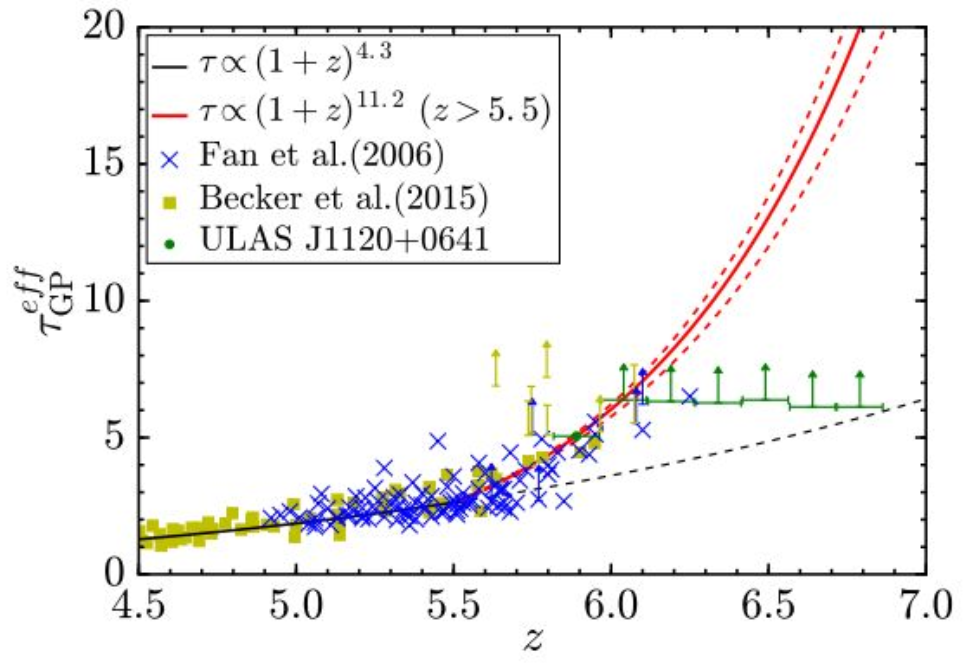
\includegraphics[width=\textwidth]{assets/gunn-peterson.png}
    \captionof{figure}{How the effective Gunn-Peterson optical depth increases with redshift, providing only a lower limit on when reionization finished.}
    \label{fig:gunn_peterson}
\end{minipage}

\subsection{Synthesis and Open Questions} \label{subsec:reionization_open}

The two main observational probes of reionization are, at first sight, in tension: QSO absorption spectra imply a substantially neutral IGM ($X_{\mathrm{HI}} > 10^{-4}$) as late as $z \sim 6$, while CMB constraints, under the simplistic assumption of instantaneous reionization, suggest a somewhat higher characteristic redshift, $z_{\text{re}} \sim 7$-$8$. The two results are, however, entirely consistent once the instantaneous approximation is relaxed: the data collectively favour an extended reionization process, beginning at $z > 8$ and completing around $z \sim 6$, rather than a single sharp transition.

\smallskip

Several fundamental questions nonetheless remain open:

\begin{itemize}
    \item The precise epoch of reionization, that is, when sources first produced enough ionising photons to complete the process, remains loosely bounded to the broad range $6 \lesssim z \lesssim 20$. 
    \item The nature of the transition, whether sudden or gradual, and whether homogeneous or highly inhomogeneous across different environments, is still actively debated. 
    \item The dominant sources of reionization, most plausibly the first generation of stars and galaxies, but with possible contributions from accreting black holes or even more exotic particle physics, are not yet firmly established.
\end{itemize}

In summary, while remarkable observational progress has transformed our understanding of cosmic reionization, the detailed timeline, physical mechanisms, and key sources remain active areas of research. Continued advances in both observations and theory are crucial to fully unravel this pivotal chapter in the history of the universe.